\documentclass[
	% -- opções da classe memoir --
	12pt,				% tamanho da fonte
	openright,			% capítulos começam em pág ímpar (insere página vazia caso preciso)
	twoside,			% para impressão em recto e verso. Oposto a oneside
	a4paper,			% tamanho do papel. 
	% -- opções da classe abntex2 --
	%chapter=TITLE,		% títulos de capítulos convertidos em letras maiúsculas
	%section=TITLE,		% títulos de seções convertidos em letras maiúsculas
	%subsection=TITLE,	% títulos de subseções convertidos em letras maiúsculas
	%subsubsection=TITLE,% títulos de subsubseções convertidos em letras maiúsculas
	% -- opções do pacote babel --
	article,	
	english,			% idioma adicional para hifenização
	french,				% idioma adicional para hifenização
	spanish,			% idioma adicional para hifenização
	brazil				% o último idioma é o principal do documento
	]{abntex2}

% ---
% Pacotes básicos 
% ---

\usepackage{lmodern}			% Usa a fonte Latin Modern			
\usepackage[T1]{fontenc}		% Selecao de codigos de fonte.
\usepackage[utf8]{inputenc}		% Codificacao do documento (conversão automática dos acentos)
\usepackage{indentfirst}		% Indenta o primeiro parágrafo de cada seção.
\usepackage{color}				% Controle das cores
\usepackage{graphicx}			% Inclusão de gráficos
\usepackage{microtype} 			% para melhorias de justificação
% ---

\usepackage{caption}
\usepackage{subcaption}

\renewcommand{\ABNTEXchapterfont}{\normalfont}	
\usepackage{mathpazo} 
% ---
% Pacotes adicionais, usados apenas no âmbito do Modelo Canônico do abnteX2
% ---
\usepackage{lipsum}				% para geração de dummy text
% ---
\usepackage{float}
%\usepackage{subfigure}
% ---
% Pacotes de citações
% ---
\usepackage[brazilian,hyperpageref]{backref}	 % Paginas com as citações na bibl
\usepackage[alf]{abntex2cite}	% Citações padrão ABNT

% --- 
% CONFIGURAÇÕES DE PACOTES
% --- 

% ---
% Configurações do pacote backref
% Usado sem a opção hyperpageref de backref
\renewcommand{\backrefpagesname}{Citado na(s) página(s):~}
% Texto padrão antes do número das páginas
\renewcommand{\backref}{}
% Define os textos da citação
\renewcommand*{\backrefalt}[4]{
	\ifcase #1 %
		Nenhuma citação no texto.%
	\or
		Citado na página #2.%
	\else
		Citado #1 vezes nas páginas #2.%
	\fi}%
% ---

% ---
% Informações de dados para CAPA e FOLHA DE ROSTO
% ---
\titulo{Eletrônica\\ Relatório de aula prática}
\autor{DOUGLAS V. BERNARDINO (EEI.180303)}
\local{Brasil}
\data{21 de agosto de 2019}
\orientador{Prof. Francisco de Assis}
\coorientador{}
\instituicao{%
  INSTITUTO FEDERAL DE EDUCAÇÃO, CIÊNCIA E TECNOLOGIA DO MARANHÃO
  \par
  DEPARTAMENTO DE ENGENHARIA}
\tipotrabalho{Tese (Doutorado)}
% O preambulo deve conter o tipo do trabalho, o objetivo, 
% o nome da instituição e a área de concentração 
\preambulo{Este trabalho é um relatório técnico de uma aula prática e o mesmo visa a obtenção de pontos na disciplina de Eletrônica.}
% ---


% ---
% Configurações de aparência do PDF final

% alterando o aspecto da cor azul
\definecolor{blue}{RGB}{41,5,195}

% informações do PDF
\makeatletter
\hypersetup{
     	%pagebackref=true,
		pdftitle={\@title}, 
		pdfauthor={\@author},
    	pdfsubject={\imprimirpreambulo},
	    pdfcreator={LaTeX with abnTeX2},
		pdfkeywords={abnt}{latex}{abntex}{abntex2}{trabalho acadêmico}, 
		colorlinks=true,       		% false: boxed links; true: colored links
    	linkcolor=blue,          	% color of internal links
    	citecolor=blue,        		% color of links to bibliography
    	filecolor=magenta,      		% color of file links
		urlcolor=blue,
		bookmarksdepth=4
}
\makeatother
% --- 

% ---
% Posiciona figuras e tabelas no topo da página quando adicionadas sozinhas
% em um página em branco. Ver https://github.com/abntex/abntex2/issues/170
\makeatletter
\setlength{\@fptop}{5pt} % Set distance from top of page to first float
\makeatother
% ---
% Possibilita criação de Quadros e Lista de quadros.


% O tamanho do parágrafo é dado por:
\setlength{\parindent}{1.3cm}

% Controle do espaçamento entre um parágrafo e outro:
\setlength{\parskip}{0.2cm}  % tente também \onelineskip
% ---
% compila o indice
% ---
\makeindex
% ---

% ----
% Início do documento
% ----
\begin{document}

% Seleciona o idioma do documento (conforme pacotes do babel)
%\selectlanguage{english}
\selectlanguage{brazil}

% Retira espaço extra obsoleto entre as frases.
\frenchspacing 

% ----------------------------------------------------------
% ELEMENTOS PRÉ-TEXTUAIS
% ----------------------------------------------------------
% \pretextual

% ---
% Capa
% ---
\imprimircapa
% ---

% ---
% Folha de rosto
% (o * indica que haverá a ficha bibliográfica)
% ---
\imprimirfolhaderosto*
% ---

% ---
% RESUMOS
% ---

% resumo em português
\setlength{\absparsep}{18pt} % ajusta o espaçamento dos parágrafos do resumo
\begin{resumo}
 No universo da eletrônica é constantemente necessário filtrar ou retificar alguns tipos de sinais. Entre uma vasta gama de retificadores, há um trivial, muito utilizado quando se precisa de uma corrente contínua tendo como fonte uma alternada, este tipo é conhecido como \emph{retificador de meia onda}, que consiste em um diodo em série com um resistor e ele será o objeto de estudo deste trabalho.

 \textbf{Palavras-chave}: retificador, meia, onda.
\end{resumo}
\newpage
% resumo em inglês
\begin{resumo}[Abstract]
 \begin{otherlanguage*}{english}
   In the universe of electronics it is constantly necessary to filter or rectify some types of signals. Among a wide range of rectifiers, there is a trivial one, widely used when one needs a direct current from an alternating source, this type is known as \emph {half wave rectifier} which consists of a diode in series with a resistor and it will be the object of study of this work.

   \vspace{\onelineskip}
 
   \noindent 
   \textbf{Keywords}: rectifier, half, wave.
 \end{otherlanguage*}
\end{resumo}


% ---
\newpage
% ---
% inserir lista de ilustrações
% ---
\newpage
% ---
% inserir o sumario
% ---
\pdfbookmark[0]{\contentsname}{toc}
\tableofcontents*
\cleardoublepage
% ---



% ----------------------------------------------------------
% ELEMENTOS TEXTUAIS
% ----------------------------------------------------------
\textual

% ----------------------------------------------------------
% Introdução (exemplo de capítulo sem numeração, mas presente no Sumário)
% ----------------------------------------------------------
\section{Retificador de meia onda}
\par Por vezes, é necessário \emph{retificar} uma corrente de forma que a mesma só atravesse o circuito em um único sentido. Para isto pode ser usado o retificador de meia onda, que nada mais é que um diodo em série com um resistor ou carga, como ilustrado na Figura 1.

\begin{figure}[H]\centering
\caption{Retificador de meia onda}
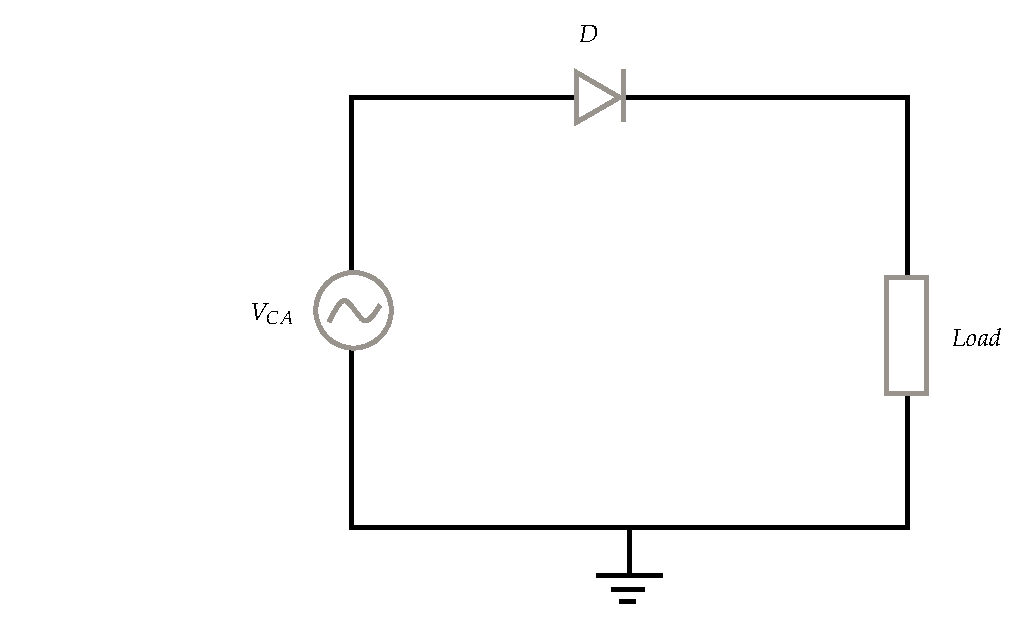
\includegraphics[trim=4cm 0cm 2mm 0cm,clip,scale=0.7]{figFinal.eps}
\begin{center}Fonte: autoria própria\end{center}
\end{figure}

\par Este circuito foi realizado durante a aula prática no Laboratório de Eletrônica, e para tal, foram usados alguns itens, listados e mostrados a seguir.


\begin{itemize}
\item $(1)$ resistor de $R = 2.2\,k\Omega$
\item $(1)$ resistor de $R = 1.2\,k\Omega$
\item $(4)$ diodo
\item $(1)$ transformador de $220V$ para $12V / 24V$
\item $(1)$ LED amarelo
\item $(1)$ LED vermelho
\item $(-)$ jumpers
\item $(1)$ protoboard
\item $(1)$ bancada de madeira
\item $(1)$ multímetro digital
\item $(1)$ osciloscópio
\end{itemize}

\par A seguir, é mostrado cada item listado acima.

\begin{figure}[H]\center
	\begin{subfigure}[H]{0.3\textwidth}\center
		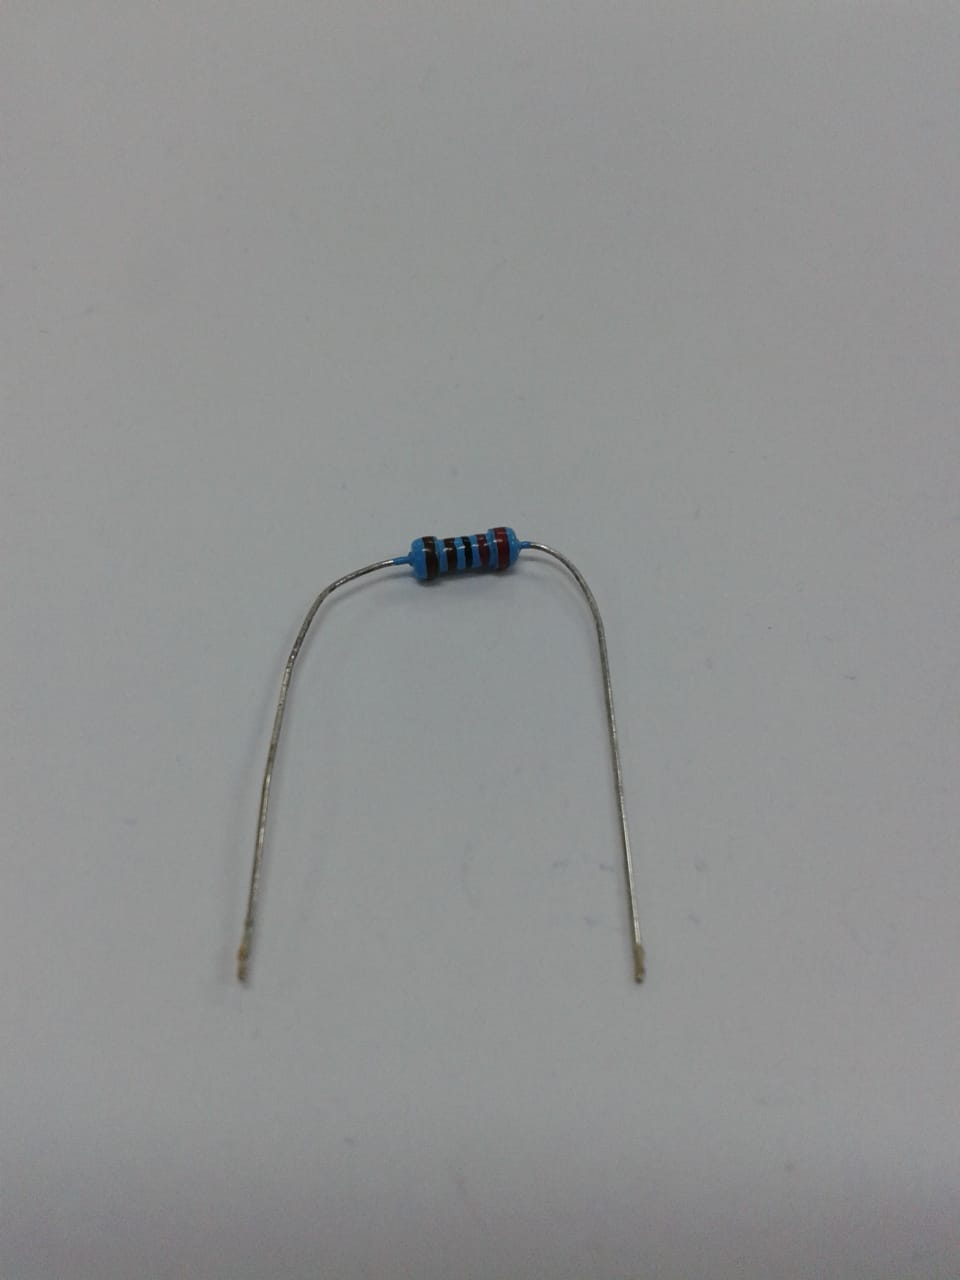
\includegraphics[trim=7cm 10cm 9cm 18cm, clip, width=\textwidth]{res22.jpeg}
		\caption{Resistor de $2.2\, k\Omega$}
	\end{subfigure}
\hfill
	\begin{subfigure}[H]{0.3\textwidth}\center
		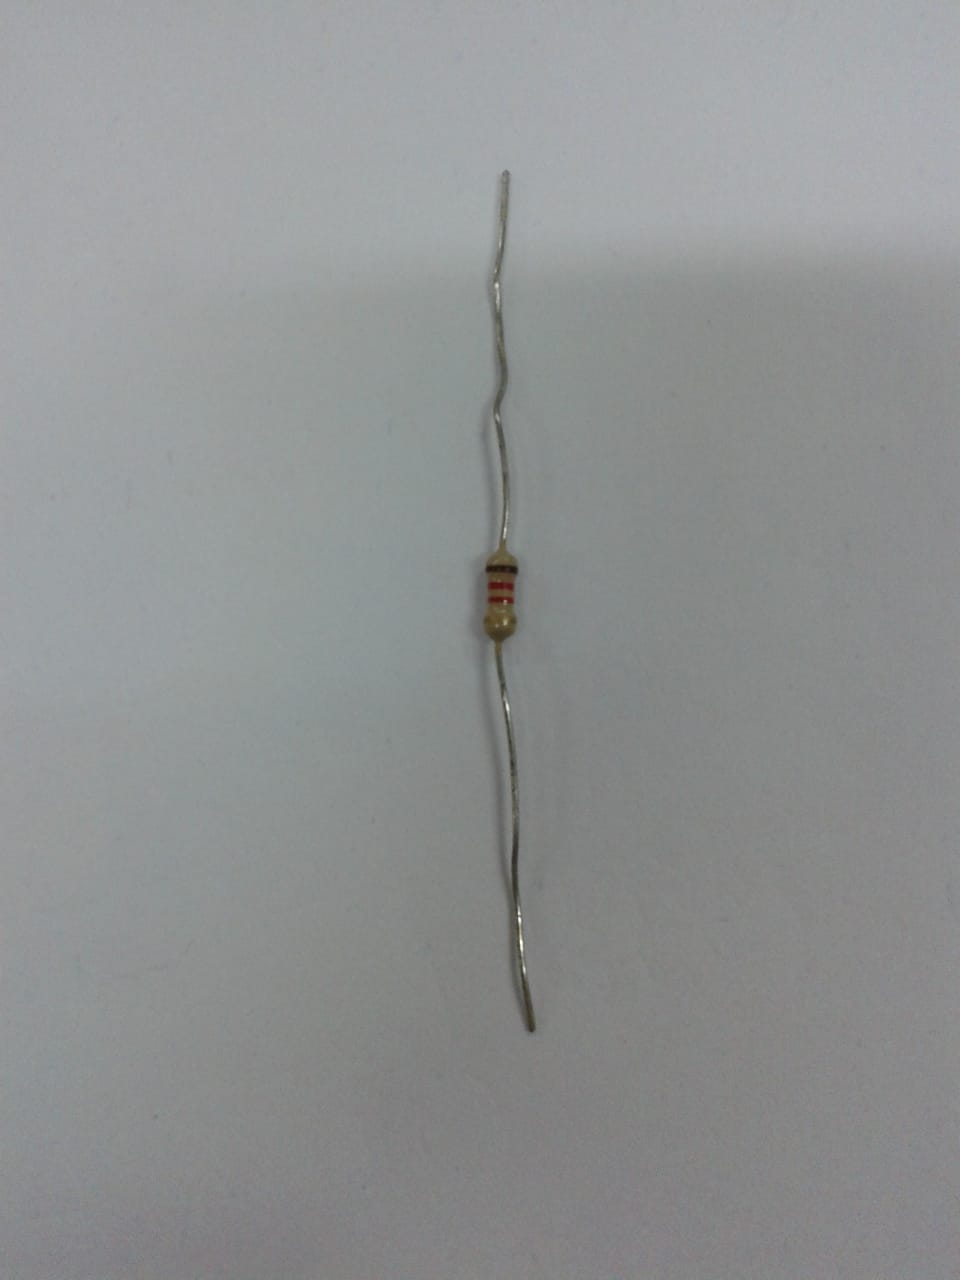
\includegraphics[trim=14cm 15cm 12cm 14cm, clip, scale=0.3]{resistor.jpeg}
		\caption{Resistor de $1.2\,k\Omega$}
	\end{subfigure}
\hfill
	\begin{subfigure}[H]{0.3\textwidth}\center
		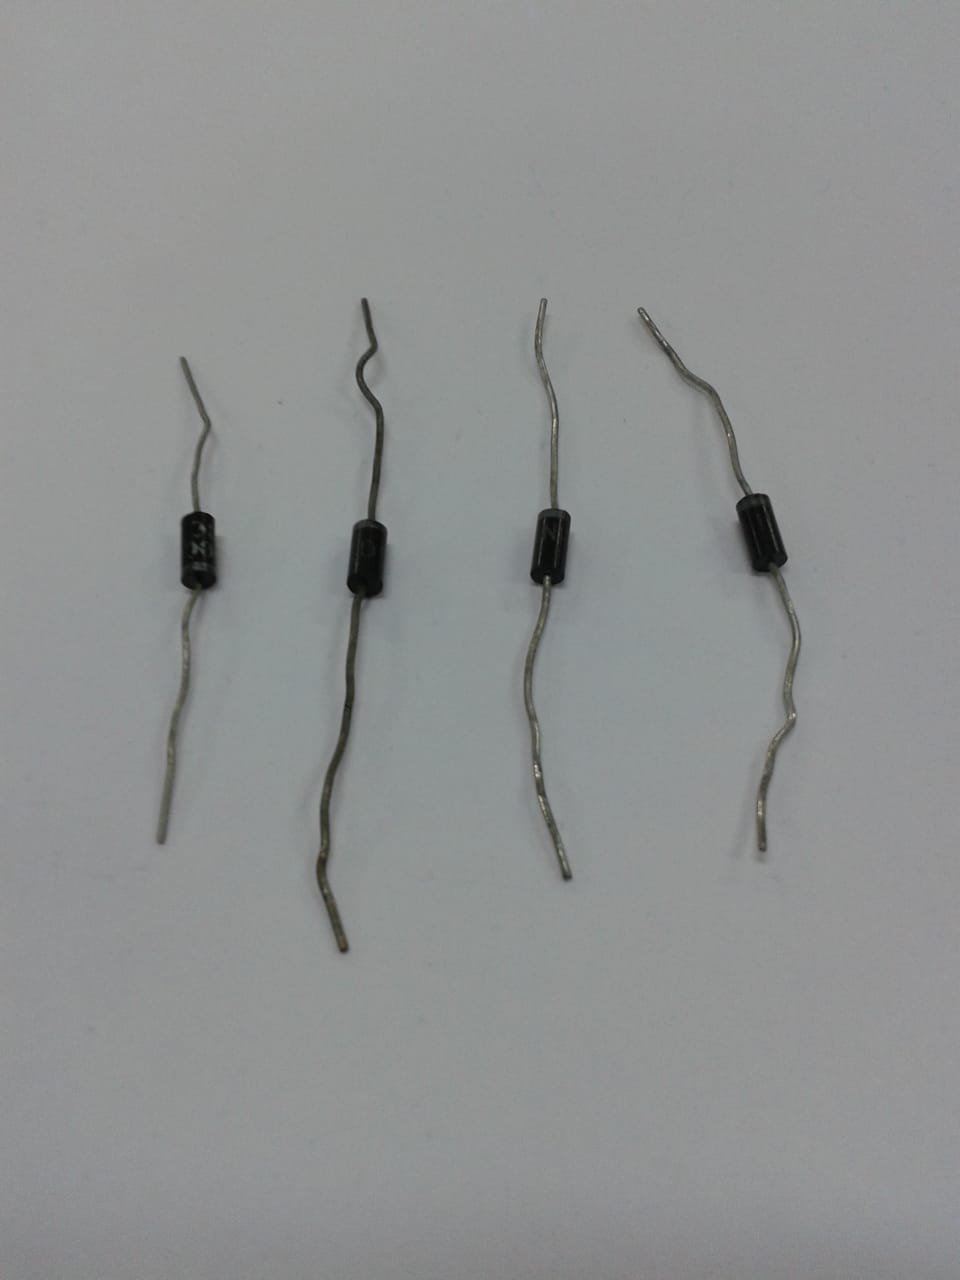
\includegraphics[trim=5cm 10cm 5cm 10cm, clip, width=\textwidth]{1.jpeg}
		\caption{Diodos}
	\end{subfigure}
\hfill
	\begin{subfigure}[H]{0.3\textwidth}\center
		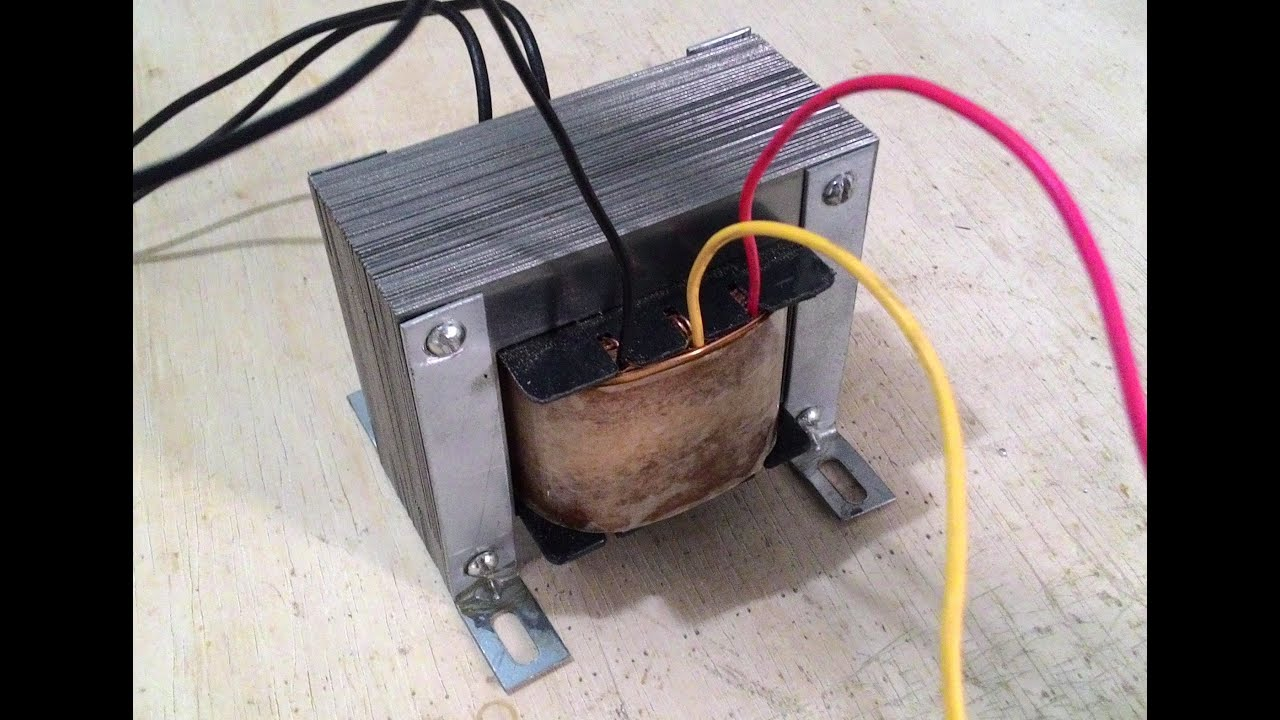
\includegraphics[trim=5cm 0 5cm 0, clip, width=\textwidth]{maxresdefault.jpg}
		\caption{Transformador}
	\end{subfigure}
\hfill
	\begin{subfigure}[H]{0.3\textwidth}\center
		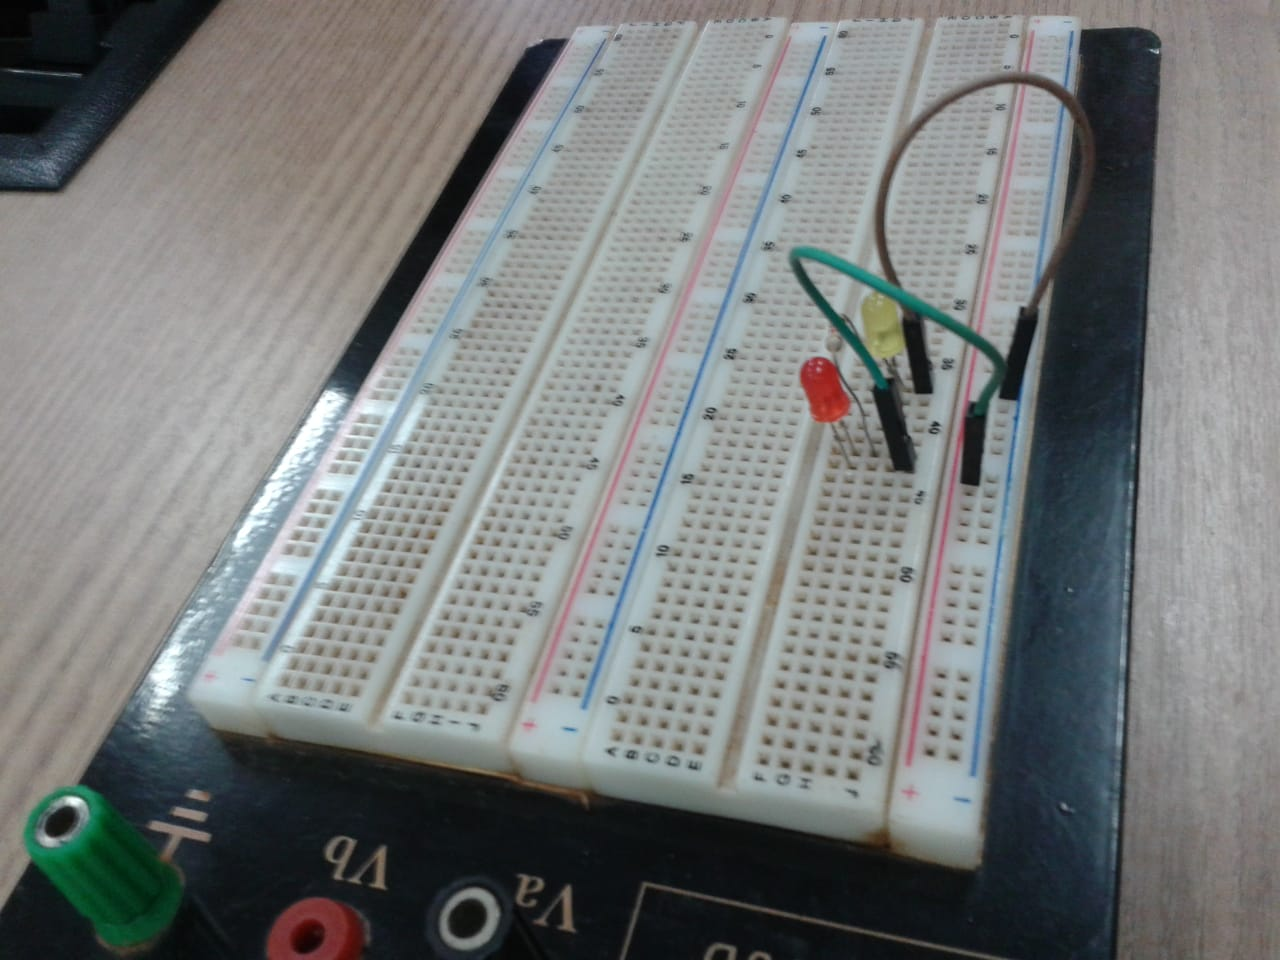
\includegraphics[trim=30cm 20.5cm 11.5cm 10cm,clip,width=\textwidth]{led(s).jpeg}
		\caption{LED amarelo}
	\end{subfigure}
\hfill
	\begin{subfigure}[H]{0.3\textwidth}\center
		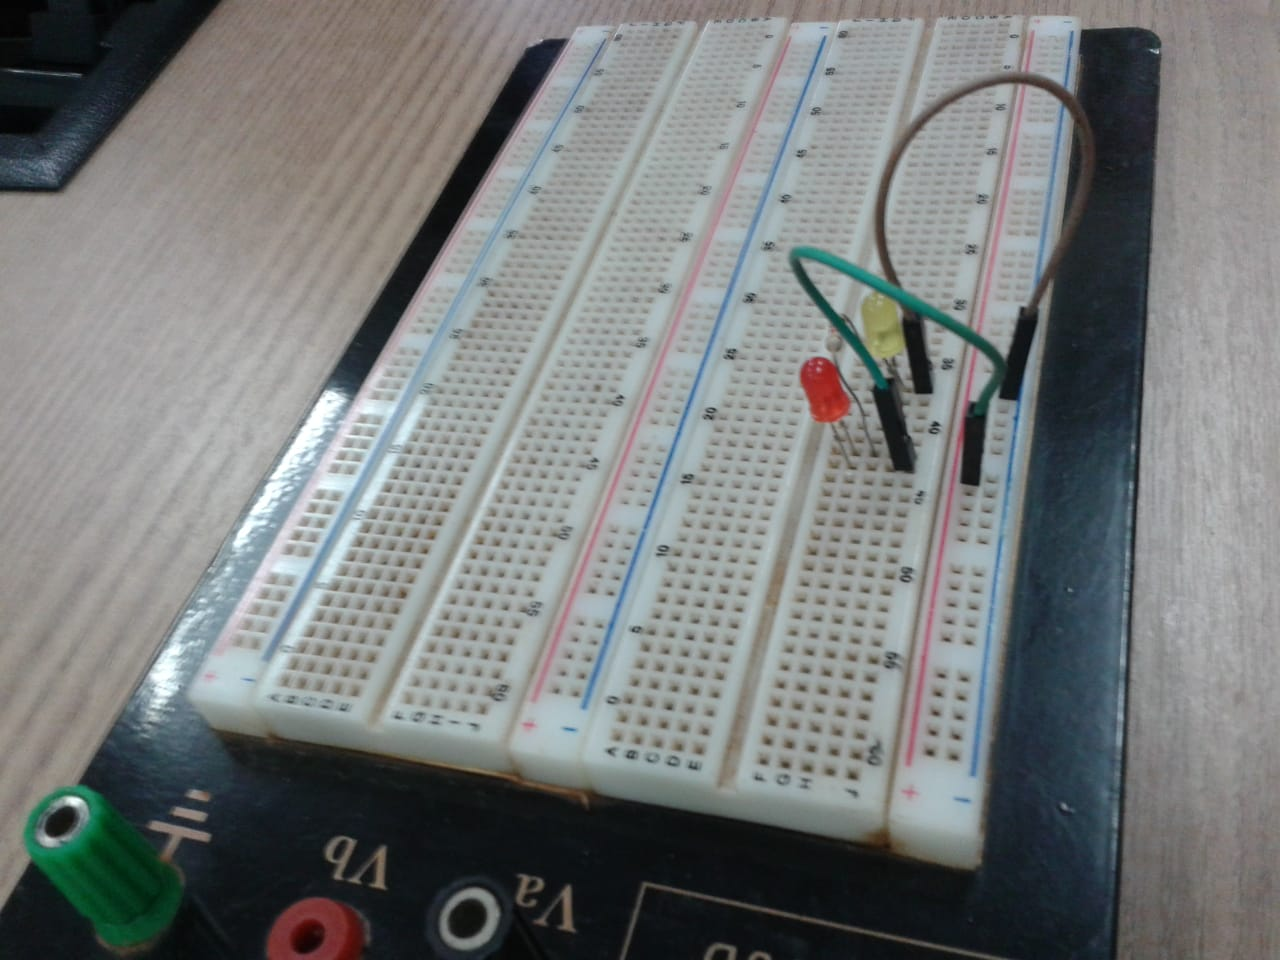
\includegraphics[trim=27cm 17.7cm 14cm 12.3cm,clip,width=\textwidth]{led(s).jpeg}
		\caption{LED vermelho}
	\end{subfigure}
\hfill
	\begin{subfigure}[H]{0.3\textwidth}\center
		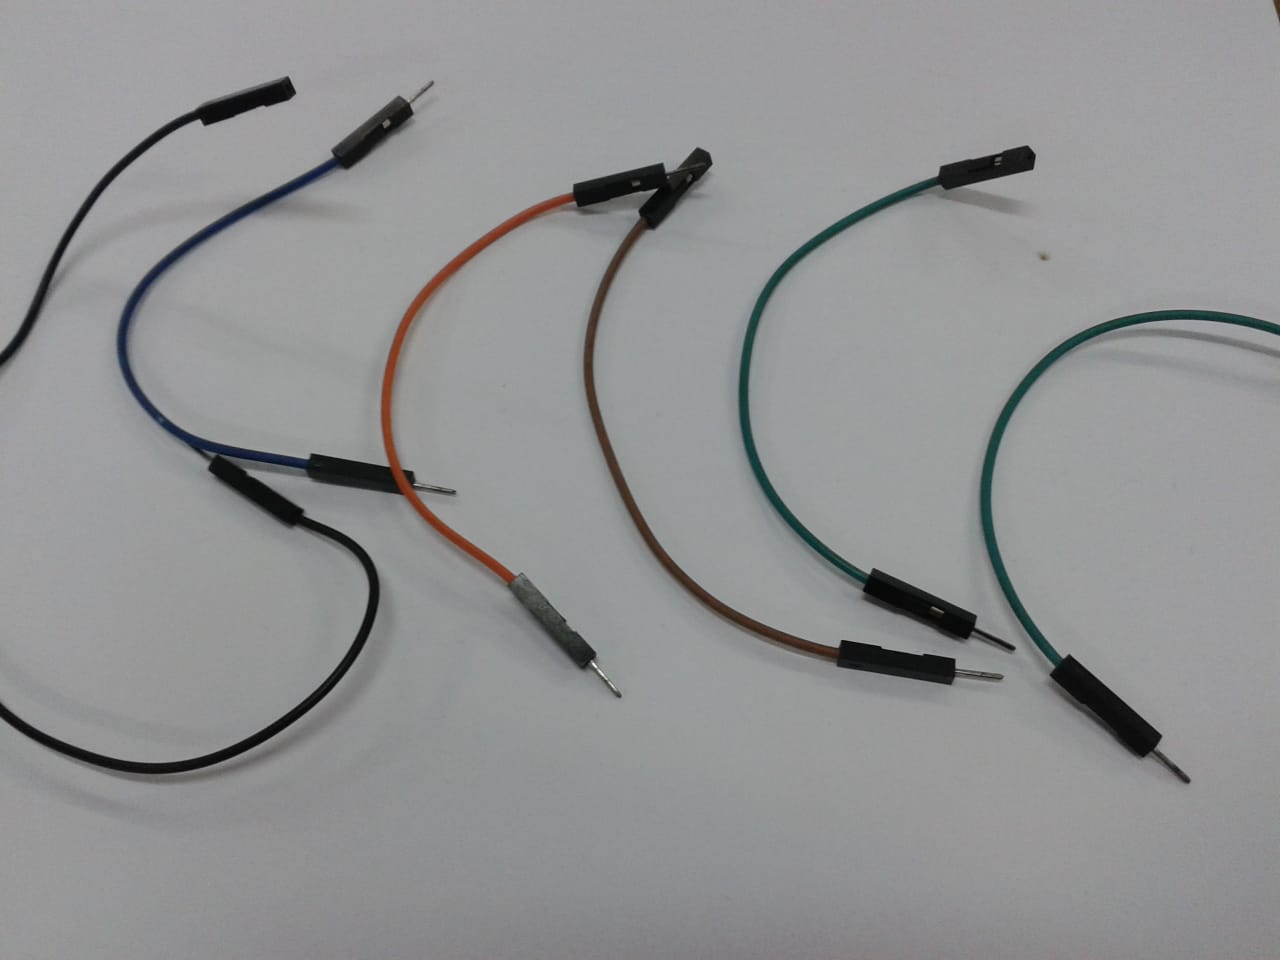
\includegraphics[width=\textwidth]{jumpers.jpeg}
		\caption{Jumpers}
	\end{subfigure}
\hfill
	\begin{subfigure}[H]{0.3\textwidth}\center
		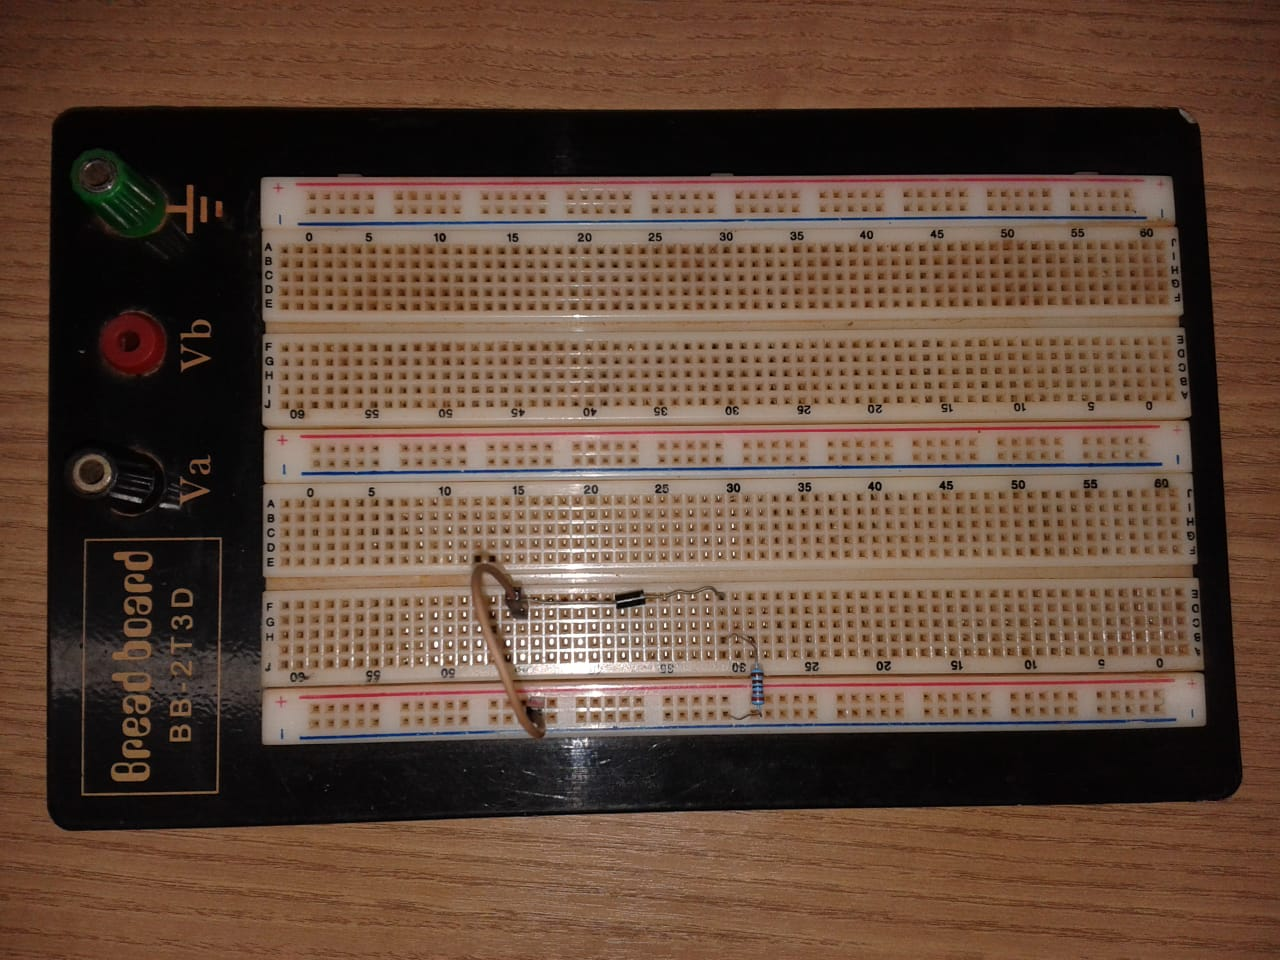
\includegraphics[width=\textwidth]{proto.jpeg}
		\caption{Protoboard}
	\end{subfigure}
\hfill
	\begin{subfigure}[H]{0.3\textwidth}\center
		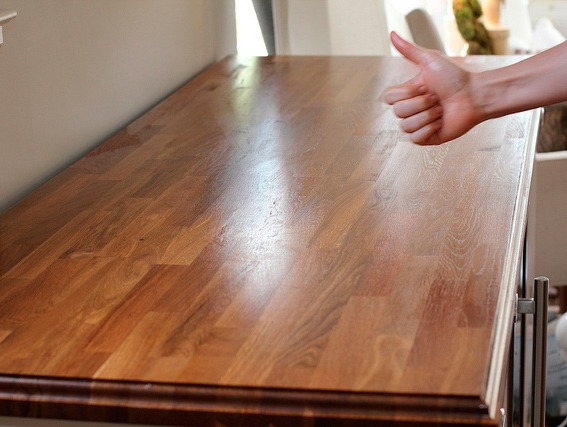
\includegraphics[trim=5cm 5cm 5cm 5cm, clip, width=\textwidth]{bancada.jpg}
		\caption{Bancada de madeira}
	\end{subfigure}
\hfill
	\begin{subfigure}[H]{0.3\textwidth}\center
		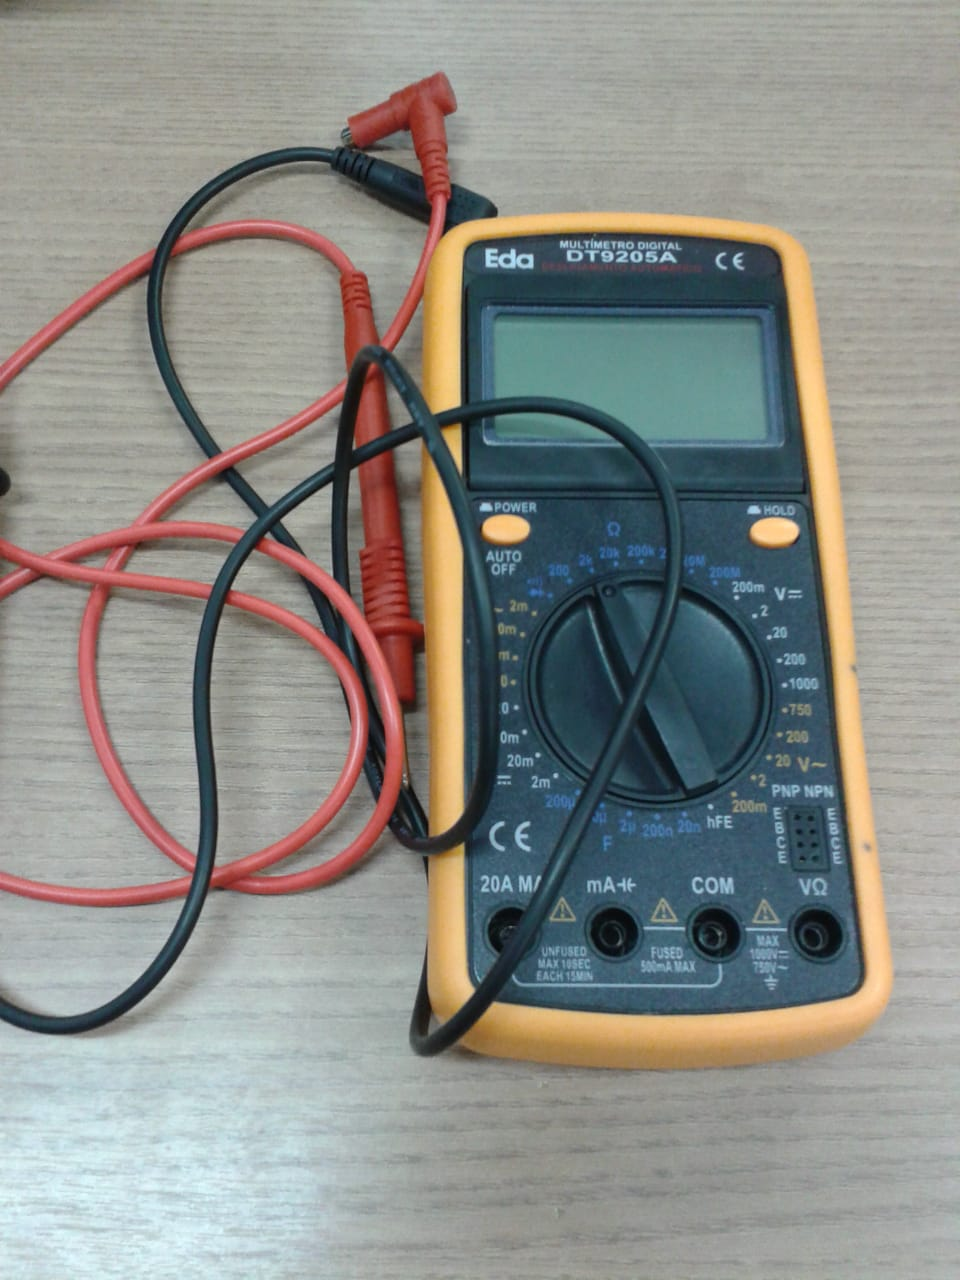
\includegraphics[angle=90, width=\textwidth]{multimetro.jpeg}
		\caption{Multímetro digital}
	\end{subfigure}
\hspace{0.5cm}
	\begin{subfigure}[H]{0.3\textwidth}\center
		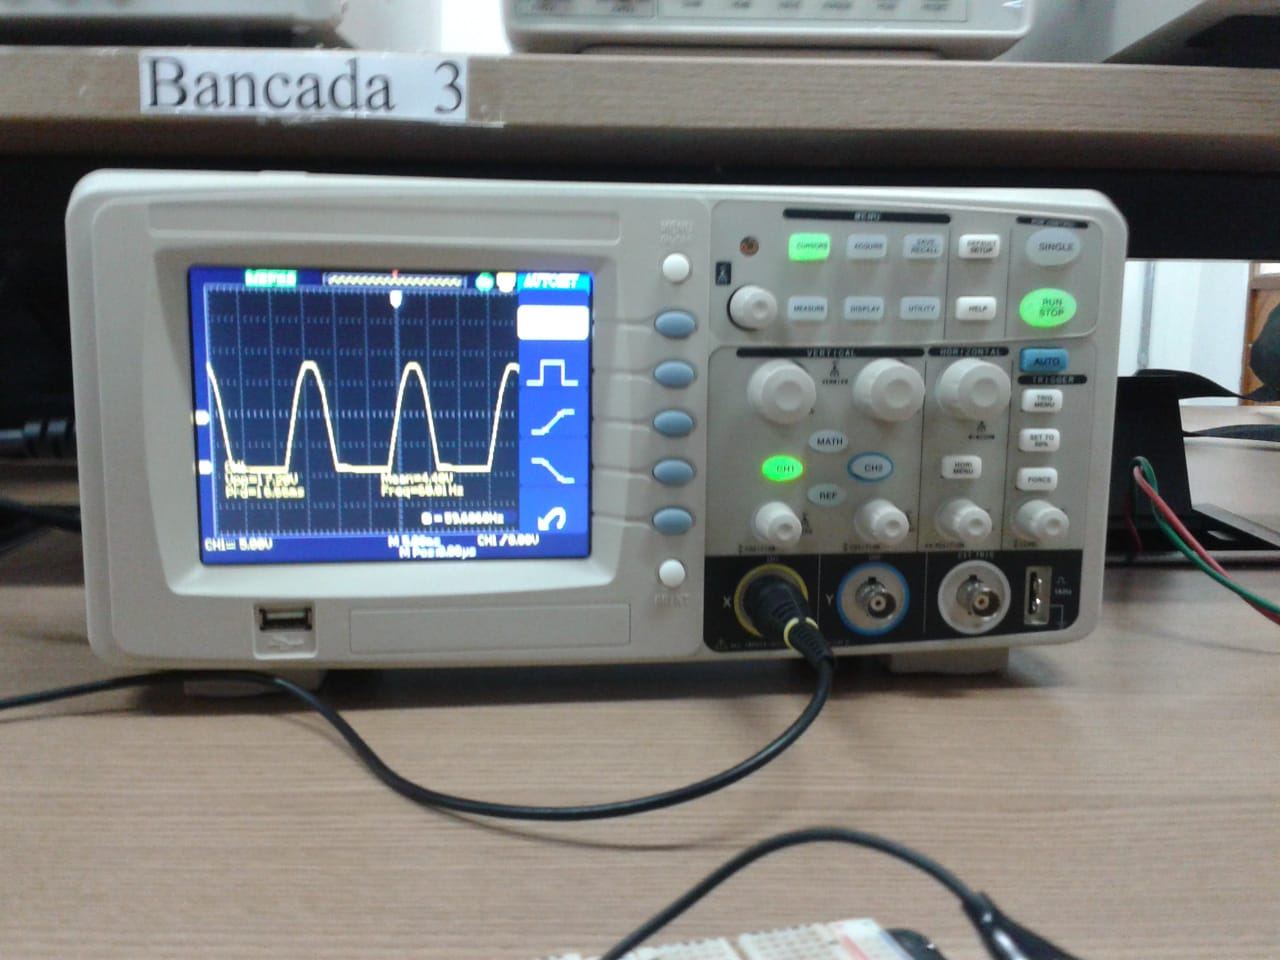
\includegraphics[width=\textwidth]{osciloscopio.jpeg}
		\caption{Osciloscópio}
	\end{subfigure}
	\caption{Itens usados na prática}
\end{figure}

\par Depois de montado, o circuito físico do retificador de meia onda fica como na Figura 3, mostrada logo abaixo.

\begin{figure}[H]\centering
\caption{Circuito físico do retificador}
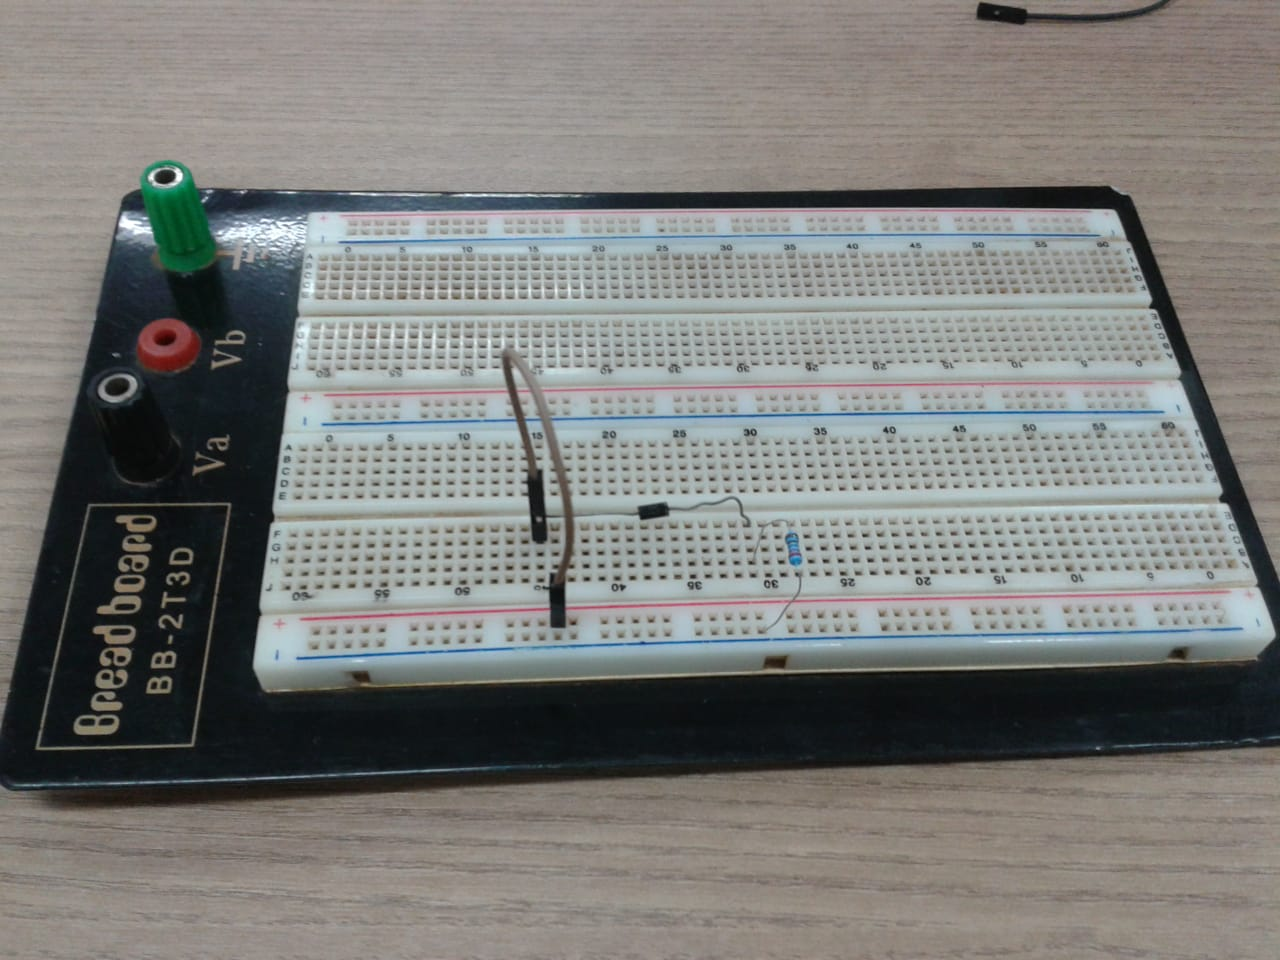
\includegraphics[scale=0.3]{circuitomontado.jpeg}

Fonte: elaboração própria
\end{figure}

\par O circuito foi alimentado com um sinal de $24 V$ alternado. A forma de onda obtida foi a mesma que a esperada, e pode ser vista na Figura 4 logo abaixo.

\begin{figure}[H]\centering
\caption{Sinal de saída do circuito retificador}
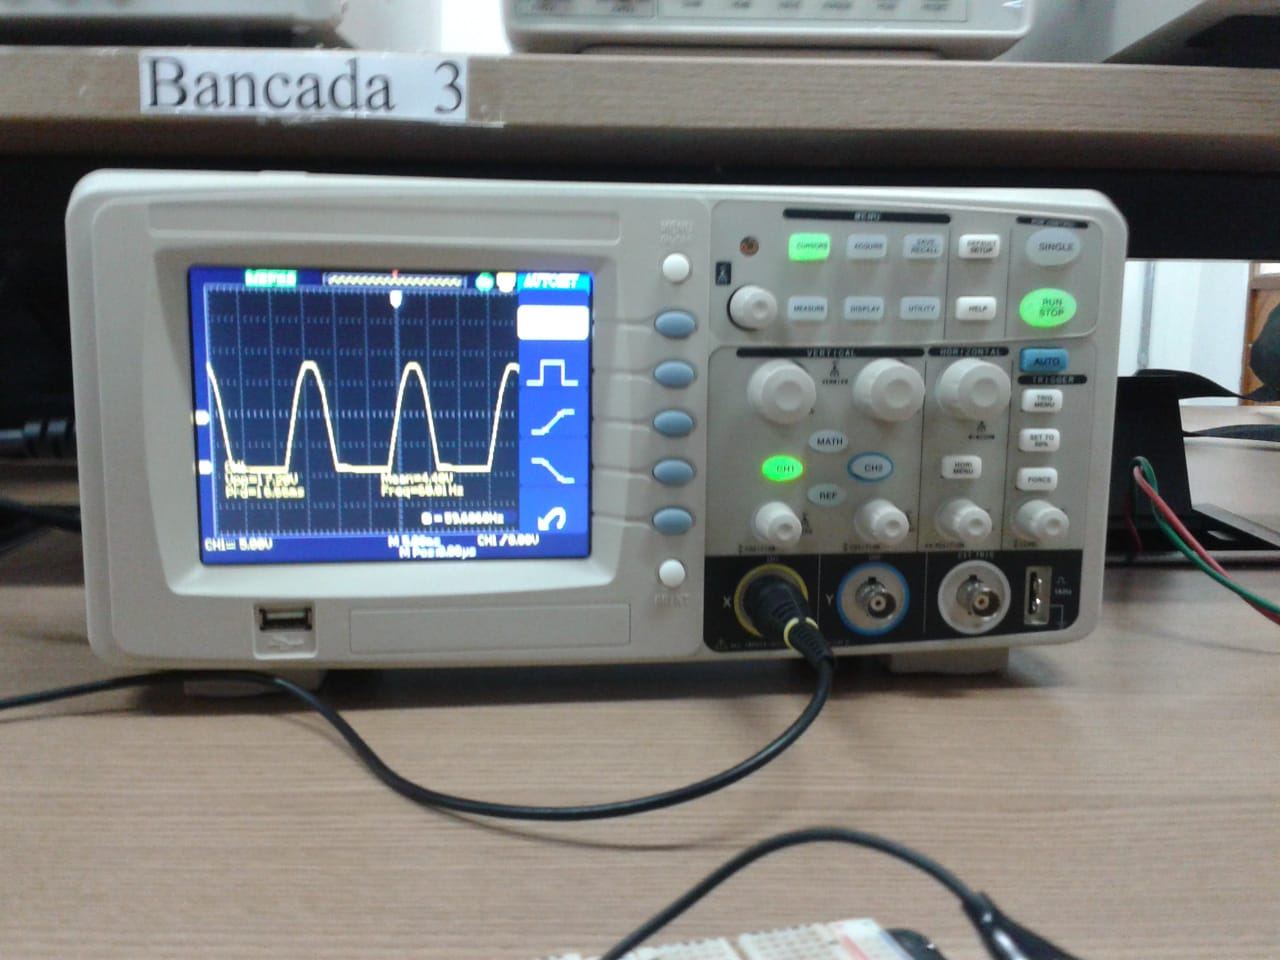
\includegraphics[scale=0.8,trim=6.5cm 14cm 24cm 9.2cm,clip]{waveform1.jpeg}

Fonte: elaboração própria
\end{figure}

\par Como se pode observar, a parte negativa do sinal foi "retirado", este é específicamente o resultado esperado do circuito retificador de meia onda. Ao inverter a polaridade, a parte positiva do sinal é "perdida" como pode ser visto na Figura 5, a seguir.

\begin{figure}[H]\centering
\caption{Sinal de saída do circuito retificador invertido}
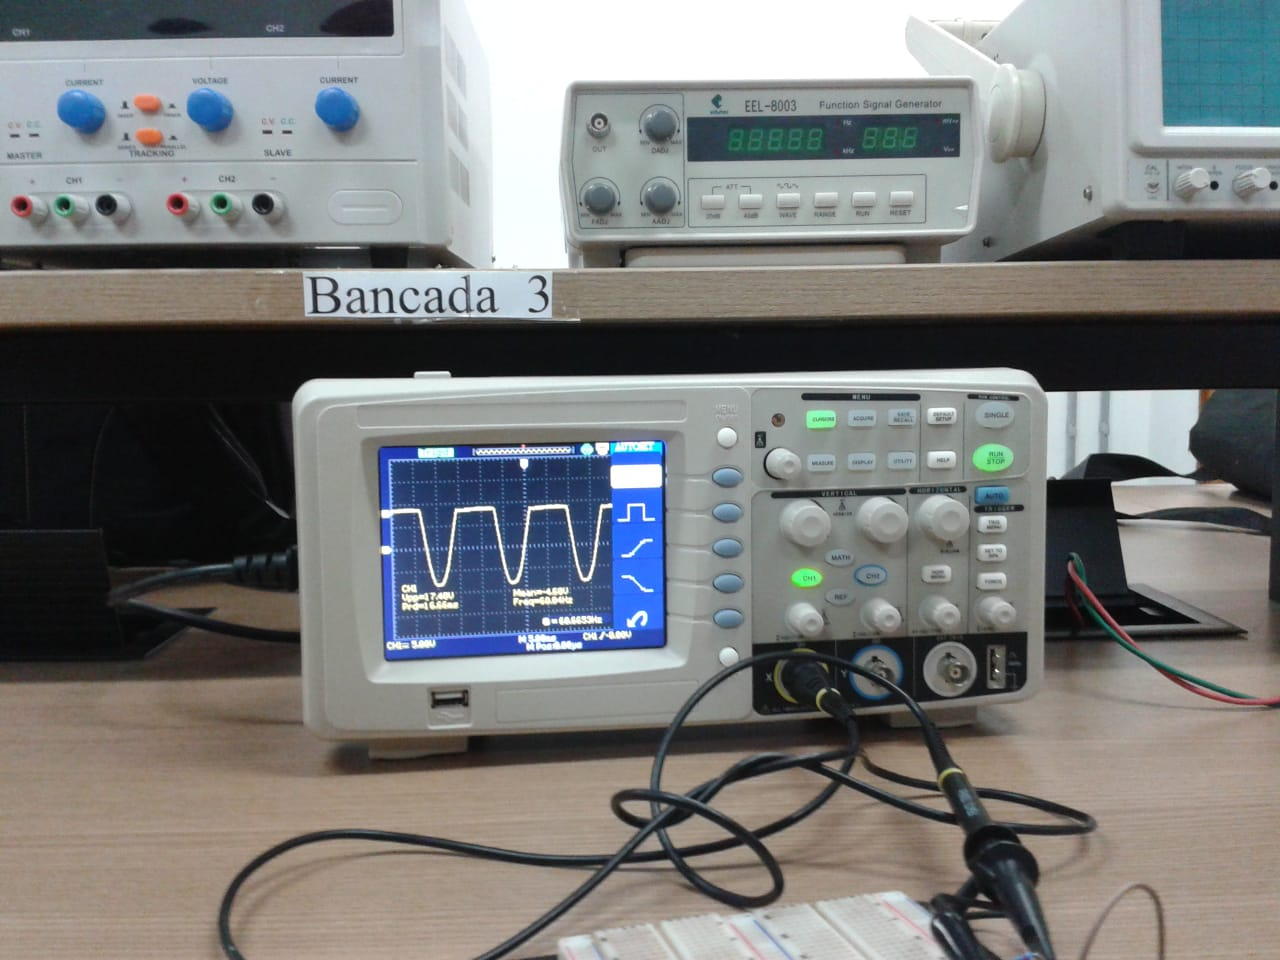
\includegraphics[scale=1.2,trim=13cm 10.5cm 21.5cm 15.3cm,clip]{waveform2.jpeg}

Fonte: elaboração própria
\end{figure}

\section{Segunda prática}
A próximo circuito testado foi o da Figura 6, mostrado logo a seguir.

\begin{figure}[H]\centering
\caption{Segundo circuito}
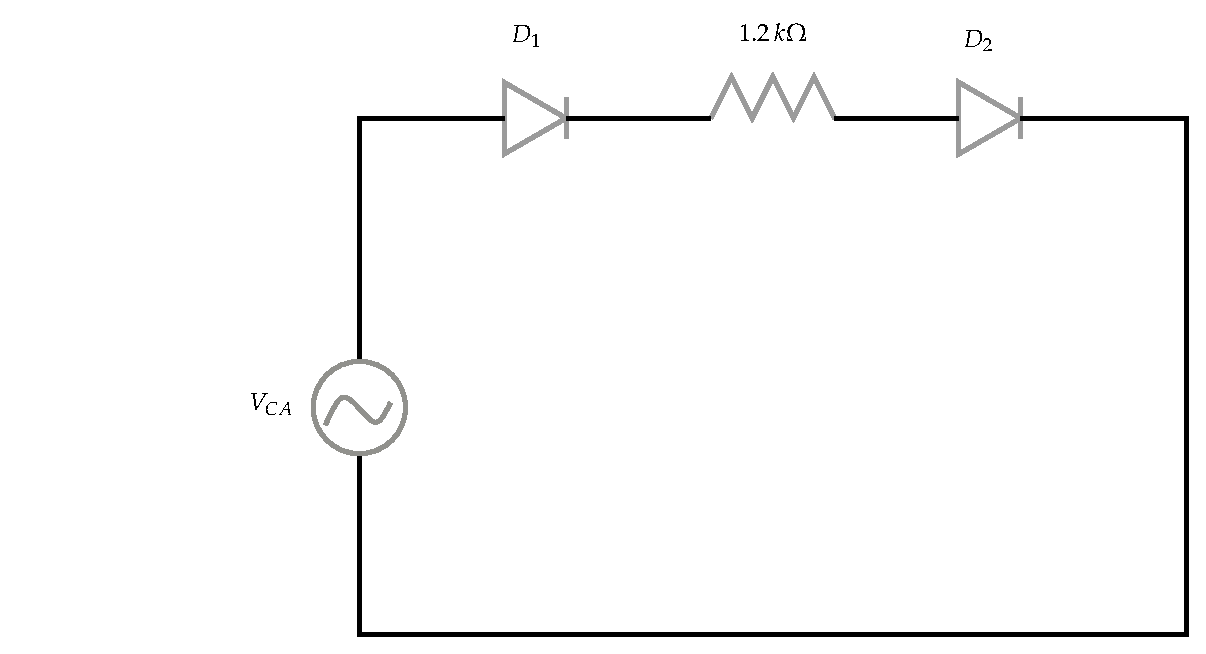
\includegraphics[trim=4cm 0 0 0, clip, scale=0.7]{ss.eps}

Fonte: autoria própria
\end{figure}

\par O circuito da Figura 6 foi realizado na prática e foi colado LEDs no lugar dos diodos. O circuito montado pode ser visto na Figura 7.

\begin{figure}[H]\centering
\caption{Segundo circuito}
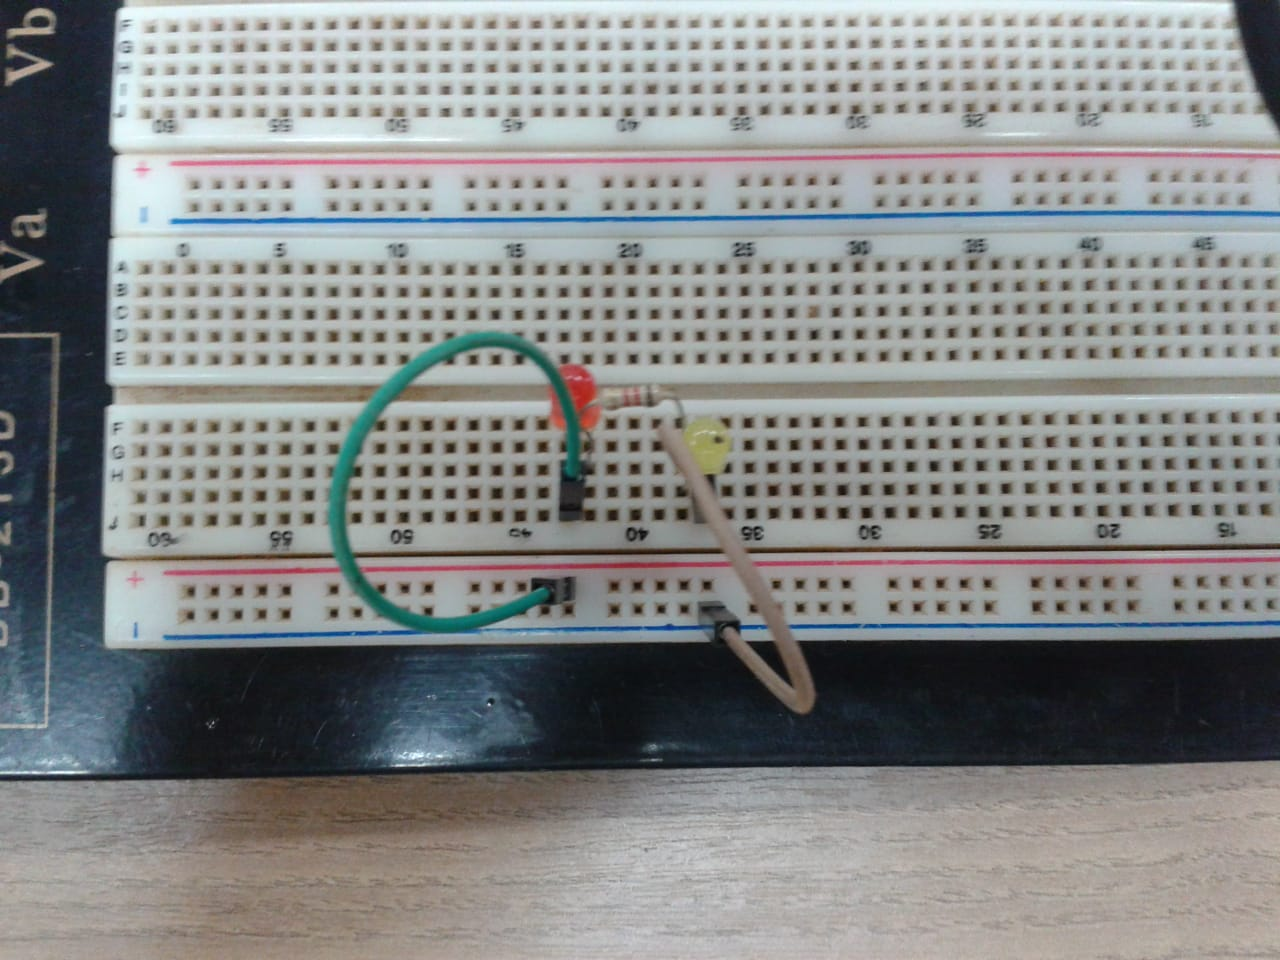
\includegraphics[scale=0.3]{circ2.jpeg}

Fonte: elaboração própria
\end{figure}

O funcionamento do circuito está enquadrado na Figura 8.

\begin{figure}[H]\centering
\caption{Segundo circuito}
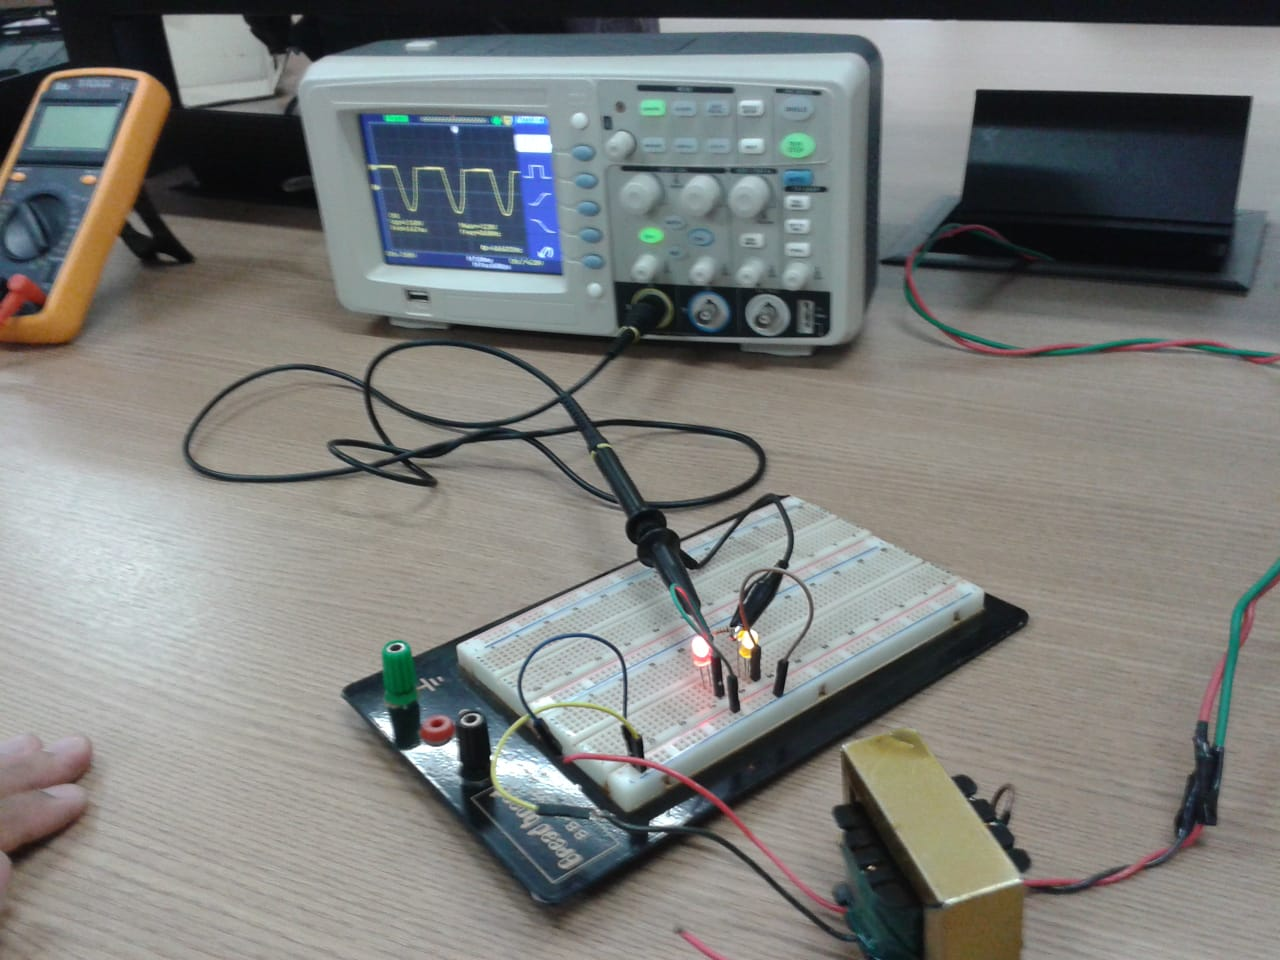
\includegraphics[scale=0.3]{adasd.jpeg}

Fonte: elaboração própria
\end{figure}

\section{Retificador em ponte}

\end{document}
